\begin{frame}{Key Concept}
\centerline{Different earth models may deliver identical measurements}
\vspace{0.2in}
\hspace{0.57in}
	\begin{tikzpicture}	
	\node at (2.0,0.0)[scale=1.03]{\begin{tikzpicture}[scale=1.5,
mipunto/.style ={color=red}]
\draw[fill=blue!70!brown] (-1.5,-1) -- (-1.5,0) -- (1.5,0) -- (1.5,-1) -- cycle;
\draw[fill=white!30!brown] (-1.5,1) -- (-1.5,0) -- (1.5,0) -- (1.5,1) -- cycle;
%\draw[line width=1.25mm,red] (0.0,0.0) -- (0.3,0.0);
\filldraw[mipunto] (0,0) circle (2.5pt);
\node (a) at (-1.,0.5) {$\rho_{1}$};  
\node (b) at (-1.,-0.5) {\textcolor{white}{$\rho_{2}$}};
\end{tikzpicture}
};
	\node at (9.0,0.0)[scale=1.03]{\input{Diapos/DL_For_Inv/Figures/Fig_field_example3.tex}};
	\end{tikzpicture}
\end{frame}

\begin{frame}{Simple example}
\centering
Simple example of an inverse problem.\\
$\qquad$\\
\begin{figure}[!htp]
	\subcaptionbox{Forward function}{%
	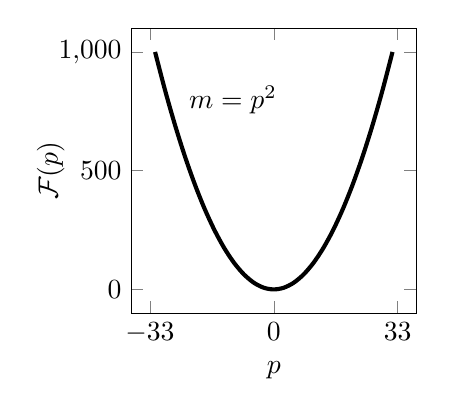
\begin{tikzpicture}
\begin{axis}
[scatter/classes={ a={mark=o,draw=blue}}, xlabel=$p$, ylabel=$ \mathcal{F}(p) $,
y label style={at={(axis description cs:-0.2,0.5)},anchor=south},
  height=5.2cm,
  width=5.2cm,
  xtick={-33,0,33}]
\addplot[smooth, line width=1.5pt, domain = -sqrt(1000):sqrt(1000), color=black] plot(\x,\x*\x) node[pos=0.1,inner sep=7pt, right] {$ m=p^2 $}; 
\end{axis}
	%\draw[->] (-3,0)--(3,0) node[right]{$x$};
	%\draw[->] (0,-2)--(0,4) node[left]{$y$};
	%\draw[smooth, line width=1.5pt, domain = -2:2, color=blue] plot(\x,\x*\x) node[right] {$ y=x^{2} $};
\end{tikzpicture}

} 
	\subcaptionbox{Inverse function with two branches}{%
	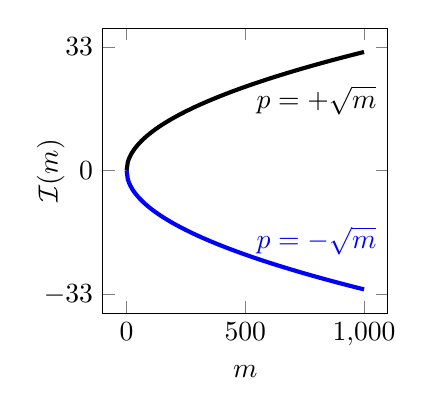
\begin{tikzpicture}
\begin{axis}
[scatter/classes={ a={mark=o,draw=blue}}, xlabel=$m$, ylabel=$\mathcal{I}(m)$,
y label style={at={(axis description cs:-0.1,0.5)},anchor=south},
  height=5.2cm,
  width=5.2cm,
  ytick={-33,0,33}]
\addplot[samples=200, line width=1.5pt, domain = 0:1000, color=black] plot(\x,{sqrt(\x)}) node[pos=0.8,inner sep=7pt, below] {$ p=+\sqrt{m} $};
\addplot[samples=200, line width=1.5pt, domain = 0:1000, color=blue] plot(\x,{-sqrt(\x)}) node[pos=0.8,inner sep=7pt, above] {$ p=-\sqrt{m} $};
\end{axis}
	%\draw[->] (-3,0)--(3,0) node[right]{$y$};
	%\draw[->] (0,-2)--(0,4) node[left]{$x$};
	%\draw[smooth, line width=1.5pt, domain = 0:3, color=blue] plot(\x,{sqrt(\x)}) node[right] {$ x=\sqrt{(x)} $};
	%\draw[smooth, line width=1.5pt, domain = 0:3, color=red] plot(\x,{-sqrt(\x)}) node[right] {$ y=-\sqrt{x} $};
\end{tikzpicture}
}
	%\caption{Model problem with known analytical solution.}
	%\label{fig:real_graphics}
\end{figure}
\end{frame}


\begin{frame}{Loss function: Data misfit}
%\vspace{-0.6 cm}
Definitions:
%\vspace{-0.2 cm}
\begin{flalign}
\hspace{3cm}
\notag
	& \mathcal{I} \;\;\:\: := \text{Inverse operator (Measurements $-->$ Earth properties)}  & \\
\notag
	& \mathcal{I}_{\phi^\ast} \: := \text{Neural Network approx. of }\mathcal{I} & 
\notag
\end{flalign}

Data misfit loss function:
\begin{flalign}
\hspace{3cm}
\notag
	 & \mathcal{I}_{\phi^\ast} \: := \arg \min_{\phi \in \Phi} \sum_i \|\mathcal{I}_{\phi}(\mathbf{m}_i)-\mathbf{p}_i\| & \\
	 \qquad
\notag
\end{flalign}
\end{frame}


\begin{frame}{Loss function: Data misfit}
\begin{figure}[!h]
\centering
	\subcaptionbox{$\left\Vert \cdot \right\Vert_{1}$-norm \label{fig:loss1_norm2}}{%
	\begin{tikzpicture}
\begin{axis}
[scatter/classes={ a={mark=o,draw=red}}, xlabel=$m$, ylabel=${\cal I}_{\theta^\ast}(m)$,
%y label style={at={(axis description cs:0.2,0.5)},anchor=south},
  legend pos=north west,
  legend style={draw=none,nodes={scale=0.5, transform shape}},
  height=5.2cm,
  width=5.2cm,
  ytick={-33,0,33}]
\addplot[scatter,only marks,%
    scatter src=explicit symbolic, color=red, mark=o]%
table[x,y] {Diapos/DL_For_Inv/Figures/Sqrt/DATA_FILES//DATA//Loss_1/Data_loss1_norm1} node[pos=.1,inner sep=7pt, above] { {\color{red} Predicted}};
%  \addlegendentry{Trained NN}
\addplot[solid,samples=200, line width=1.5pt, domain = 0:1100, color=black] plot(\x,{sqrt(\x)}) node[pos=0.7,inner sep=5pt, below] { {\color{black} Real}}; 
%  \addlegendentry{Ground Truth}
\addplot[solid,samples=200, line width=1.5pt, domain = 0:1100, color=black] plot(\x,{-sqrt(\x)});
\end{axis}
%\node at (1.65,4.2) {$L_1$ Norm};
\end{tikzpicture}



  
  
  
  
  
  
%\begin{tikzpicture}
%\begin{axis}
%[scatter/classes={ a={mark=o,draw=red}}, xlabel=$y$, ylabel=$\mathcal{I}_{h}(y)$,
%y label style={at={(axis description cs:0.2,0.5)},anchor=south},
%  height=5.8cm,
%  width=5.8cm,]
%\addplot[scatter,only marks,%
%    scatter src=explicit symbolic, color=red, mark=o]%
%table[x,y] {DATA_FILES//DATA//Loss_1//Data_loss1_norm1};
%\addplot[smooth, line width=1.5pt, domain = 0:1000, color=blue] plot(\x,{sqrt(\x)}); \label{legend:l1}
%\addplot[smooth, line width=1.5pt, domain = 0:1000, color=blue] plot(\x,{-sqrt(\x)});
%\end{axis}
%\end{tikzpicture}
}
	\hspace{0.3cm}
	\subcaptionbox{$\left\Vert \cdot \right\Vert_{2}$-norm \label{fig:loss1_norm1}}{%
	\input{Diapos/DL_For_Inv/Figures/Sqrt/Fig_loss1_norm2.tex}}
	%\caption{Analytical solution vs DNN predicted solution evaluated over the test dataset using the loss function based on the data misfit.}
	%\label{fig:loss1}
\end{figure}
\end{frame}


\begin{frame}[t]{$|| \cdot ||_2$-norm}
\visible<1-4>{For every sample of the form $(m_i,p_i)=(m_i, \sqrt{m_i})$, there exists another one $(m_i, -\sqrt{m_i})$.}
\vspace{0.3cm}

\visible<2-4>{Then, for a specific sample $m$, the solution that minimizes the loss must satisfy
\begin{equation}
(\mathcal{I}_{{\cal R},\theta}(m) - \sqrt{m})^2 + (\mathcal{I}_{{\cal R},\theta}(m) - (-\sqrt{m}))^2.
\label{eq:norm2_proof_2}
\end{equation}}

\visible<3-4>{Taking the derivative of Eq. (\ref{eq:norm2_proof_2}) with respect to $\mathcal{I}_{{\cal R},\theta}(m)$ and equaling it to zero, we obtain
\begin{equation}
4\cdot\mathcal{I}_{{\cal R},\theta}(m)= 0.
\label{eq:loss1_norm2_derived}
\end{equation}}

\visible<4-4>{Thus, for any sample $m_i$, the function is minimized when the approximated value is $\mathcal{I}_{{\cal R},\theta}(m_i)=0$.}
\end{frame}


\begin{frame}{Loss function: Desired}
%\vspace{-0.6 cm}

Definitions:
%\vspace{-0.2 cm}
\begin{flalign}
\hspace{3cm}
\notag
	& \mathcal{F} \;\;\: := \text{Forward operator (Earth properties $-->$ Measurements)}  & \\
\notag
	& \mathcal{I} \;\;\:\: := \text{Inverse problem (Measurements $-->$ Earth properties)}  & \\
\notag
	& \mathcal{I}_{\phi^\ast} \: := \text{Neural Network approx. of }\mathcal{I} & 
\notag
\end{flalign}

Desired loss function:
\begin{flalign}
\hspace{3cm}
\notag
	 & \mathcal{I}_{\phi^\ast} \: := \arg \min_{\phi \in \Phi} \sum_i \|(\mathcal{F} \circ \mathcal{I}_{\phi})(\mathbf{m}_i)-\mathbf{m}_i \| & \\
	 \qquad
\notag
\end{flalign}

\visible<2>{\centerline{\textcolor{red}{Evaluating $\mathcal{F}$  is expensive}}}
\end{frame}


\begin{frame}{Loss function: Encoder-Decoder}
%\vspace{-0.6 cm}

Definitions:
%\vspace{-0.2 cm}
\begin{flalign}
\hspace{3cm}
\notag
	& \mathcal{F} \;\;\: := \text{Forward operator (Earth properties $-->$ Measurements)}  & \\
\notag
	& \mathcal{I} \;\;\:\: := \text{Inverse operator (Measurements $-->$ Earth properties)}  & \\
\notag
	& \mathcal{F}_{\theta^\ast}:= \text{Neural Network approx. of }\mathcal{F} & \\
	& \mathcal{I}_{\phi^\ast} \: := \text{Neural Network approx. of }\mathcal{I} & 
\notag
\end{flalign}

Encoder-Decoder loss function:
\begin{flalign}
\hspace{3cm}
\notag
	 \{ \mathcal{I}_{\phi^\ast},\mathcal{F}_{\theta^\ast} \}:= & \arg \min_{\shortstack{$\scriptstyle \theta \in \Theta$ \\ $\scriptstyle \phi \in \Phi$}}  \sum_i ( \|(\mathcal{F}_{\theta} \circ \mathcal{I}_{\phi})(\mathbf{m}_i)-\mathbf{m}_i \|  + \|{\cal F}_{\theta}(\mathbf{p}_i)-\mathbf{m}_i \| )& \\
%	 & + \|{\cal F}_{\theta}(\mathbf{z}_i)-\mathbf{m}_i \| ) &
\notag
\end{flalign}
\end{frame}


\begin{frame}{Loss function: Encoder-Decoder}
\begin{figure}[!h]
\centering
	\subcaptionbox{$\left\Vert \cdot \right\Vert_{1}$-norm \label{fig:loss1_norm2}}{%
	\input{Diapos/DL_For_Inv/Figures/Sqrt/Fig_loss4_norm1_INV.tex}}
	\hspace{0.3cm}
	\subcaptionbox{$\left\Vert \cdot \right\Vert_{2}$-norm \label{fig:loss1_norm1}}{%
	\begin{tikzpicture}
\begin{axis}
[scatter/classes={ a={mark=o,draw=red}}, xlabel=$m$, ylabel=$ {\cal I}_{\theta^\ast}(m) $,
%y label style={at={(axis description cs:0.2,0.5)},anchor=south},
  legend pos=north west,
  legend style={draw=none,nodes={scale=0.5, transform shape}},
  height=5.2cm,
  width=5.2cm,
  ytick={-33,0,33}]
\addplot[scatter,only marks,%
    scatter src=explicit symbolic, color=red, mark=o]%
table[x,y] {Diapos/DL_For_Inv/Figures/Sqrt/DATA_FILES//DATA//Loss_4//Norm_2//Data_INV_loss4_norm2} node[pos=.1,inner sep=12pt, below] { {\color{red} Predicted}};
%  \addlegendentry{Trained NN}
\addplot[solid,samples=200, line width=1.5pt, domain = 0:1100, color=black] plot(\x,{sqrt(\x)}); 
%  \addlegendentry{Ground Truth}
\addplot[solid,samples=200, line width=1.5pt, domain = 0:1100, color=black] plot(\x,{-sqrt(\x)}) node[pos=0.7,inner sep=5pt, above] { {\color{black} Real}};
\end{axis}
%\node at (1.65,4.2) {$L_2$ Norm};
\end{tikzpicture}
}
	%\caption{Analytical solution vs DNN predicted solution evaluated over the test dataset using the loss function based on the data misfit.}
	%\label{fig:loss1}
\end{figure}
\end{frame}


\begin{frame}{Loss function: Two-Step}
%\vspace{-0.6 cm}
Definitions:
%\vspace{-0.2 cm}
\begin{flalign}
\hspace{3cm}
\notag
	& \mathcal{F} \;\;\: := \text{Forward operator (Earth properties $-->$ Measurements)}  & \\
\notag
	& \mathcal{I} \;\;\:\: := \text{Inverse operator (Measurements $-->$ Earth properties)}  & \\
\notag
	& \mathcal{F}_{\theta^\ast}:= \text{Neural Network approx. of }\mathcal{F} & \\
	& \mathcal{I}_{\phi^\ast} \: := \text{Neural Network approx. of }\mathcal{I} & 
\notag
\end{flalign}

Two-step loss function:
\begin{flalign}
\hspace{3cm}
\notag
	& \mathcal{F}_{\theta^\ast}:= \arg \min_{\theta \in \Theta}  \sum_i \|{\cal F}_{\theta}(\mathbf{p}_i)-\mathbf{m}_i \| & \\
	 & \mathcal{I}_{\phi^\ast} \: := \arg \min_{\phi \in \Phi} \sum_i \|(\mathcal{F}_{\theta^\ast} \circ \mathcal{I}_{\phi})(\mathbf{m}_i)-\mathbf{m}_i \| &
\notag
\end{flalign}
\end{frame}


\begin{frame}{Loss function: Two-Step}
\begin{figure}[!h]
\centering
	\subcaptionbox{$\left\Vert \cdot \right\Vert_{1}$-norm \label{fig:loss1_norm2}}{%
	\input{Diapos/DL_For_Inv/Figures/Sqrt/Fig_loss5_norm1_INV.tex}}
	\hspace{0.3cm}
	\subcaptionbox{$\left\Vert \cdot \right\Vert_{2}$-norm \label{fig:loss1_norm1}}{%
	\input{Diapos/DL_For_Inv/Figures/Sqrt/Fig_loss5_norm2_INV.tex}}
	%\caption{Analytical solution vs DNN predicted solution evaluated over the test dataset using the loss function based on the data misfit.}
	%\label{fig:loss1}
\end{figure}
\end{frame}


